\chapter{Credit Default Swaps}

\section{Credit curves}\label{credit-curves}

Just like a discount curve is a way of representing the underlying
interest rates implicit in the market quotes of a collection of
real-world interest rate products, \textbf{credit curves} are a way of
representing the data implied by credit default swaps.

\textbf{Credit default swaps} (\textbf{CDS}) are instruments whose value
depends on the likelihood that a given company (the curve's
\textbf{issuer}) will suffer a credit event over a given period.

A \textbf{credit event} can be a default, the failure to make payments,
the issuer entering into bankruptcy proceedings, or the occurence of
other legal events. The exact definition of what constitutes a credit
event depends on a series of factors and is usually defined in some kind
of ISDA (International Swaps and Derivatives Association) master
agreement.

In any case, we will generically call a credit event a \emph{default},
and talk about \textbf{non-default probabilities} (\textbf{NDP}, or
survival probability), i.e.~the probability that the issuer will
not suffer a credit event \textbf{before} a given value date.

NDPs are the equivalent for credit curves of discount factors for
discount curves. Just like discount curves, credit curves are built by
specifying a pricing/observation date, a sequence of pillar dates and a
sequence of NDPs. We will then implement a \texttt{CreditCurve} class
that provides a method which interpolates these pillar NDPs
to return the NDP at an arbitrary value date.

In addition, we'll also write a method which returns the \textbf{hazard
rate} at an arbitrary value date. The hazard rate is the credit curve
equivalent of the short rate or overnight rate for discount curves. It
represents the instantaneous probability of the issuer defaulting
conditioned on it not having defaulted until that moment (in
practice we'll calculate it numerically, and therefore it'll be the, annualised,
conditional probability of the issuer defaulting between
the value date and the day after.

\begin{center}
  \begin{tabular}{|| c | c ||}
    \hline
    Discount Curve & Credit Curve \\
    \hline \hline
    \begin{tabular}{@{}c@{}}underlying rates implicit in \\ market quotes of IR products\end{tabular} &
    \begin{tabular}{@{}c@{}}default probabilities implied \\ by credit default swaps \end{tabular} \\
    \hline
    discount factors & non-default probabilities \\
    \hline
    short rate & hazard rate \\
    \hline  
  \end{tabular}
\end{center}

\subsection{Hazard Rate}\label{hazard-rate}

Hazard rate is often called a \emph{conditional failure rate} since it's
expression is a direct application of the conditional probability
concept.

Conditional probability answers to the question ``how should you update
probabilities of events when there is additional information available
?''. To derive the general formula let's start with an example.

A fair die is rolled. Let \(A\) be the event that the outcome is an odd
number (\(A={1,3,5}\)). Also let \(B\) be the event that the outcome is
less than or equal to \(3\) (\(B={1,2,3}\)). What is the probability of
\(A\) (\(P(A)\)) ? What is the probability of \(A\) given \(B\)
(\(P(A|B)\)) ?

Being a simple example we can compute the result by hand:

\[P(A) = \cfrac{|A|}{|S|} = \cfrac{|\{1,3,5\}|}{6} = \cfrac{1}{2}\;\;\textrm{(where S is the entire sample space)}\]

Now let's find the conditional probability of \(A\) given that \(B\)
occurred. If we know \(B\) has occurred, the outcome must be among
\(\{1,2,3\}\). For \(A\) to also happen the outcome must be in
\(A\cap B = \{1,3\}\). Since all die rolls are equally likely, we argue
that \(P(A|B)\) must be equal to

\[P(A|B) = \cfrac{|A\cap B|}{|B|} = \cfrac{2}{3}\]

To generalise our example we can rewrite the calculation by dividing the
numerator and denominator by the entire space of the events \(|S|\)
hence:

\[P(A|B) = \cfrac{|A\cap B|}{|B|} = \cfrac{\cfrac{|A\cap B|}{|S|}}{\cfrac{|B|}{|S|}} = \cfrac{P(A\cap B)}{P(B)}\]

\begin{figure}[tb]
\centering
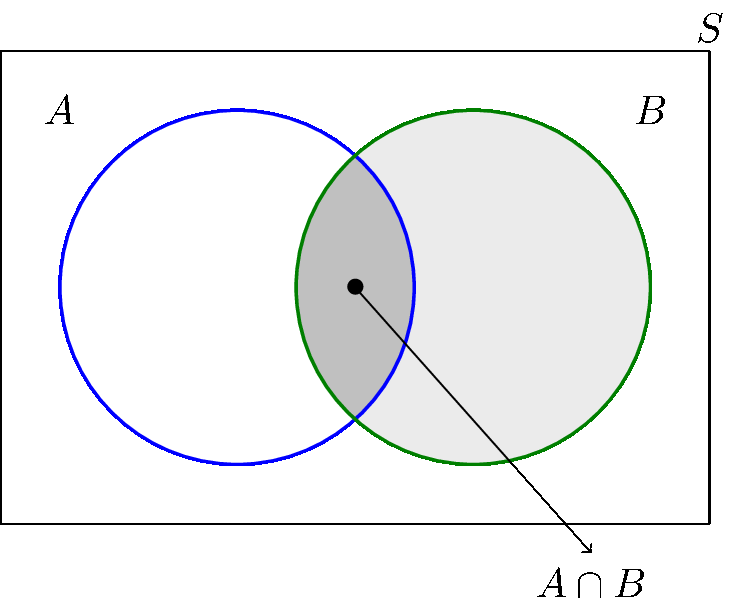
\includegraphics[width=0.7\linewidth]{conditional_b.png}
\caption{Graphical representation of conditional probability (the grey shaded area).}
\end{figure}

In formula if the non-default probability is indicated by \(N\) and the
hazard rate by \(\lambda\):

\[\lambda = \cfrac{P(\tau\in (t, t+dt))}{P(\tau>t)} = \cfrac{\cfrac{d(1-N)}{dt}}{N(t_0, t_1)} = -\cfrac{dN}{dt}\cdot\frac{1}{N(t_0, t_1)}.\]
Conversely given the hazard rate the non-default probability can be
determined as:

\[\lambda = -\cfrac{1}{dt}\cdot\cfrac{dN}{N} = -\cfrac{d(\textrm{log}N)}{dt} \implies N(t_0, t) = e^{-\int_{t_0}^{t}\lambda dt}\]

\begin{tcolorbox}[breakable, size=fbox, boxrule=1pt, pad at break*=1mm,colback=cellbackground, colframe=cellborder]
\begin{Verbatim}[commandchars=\\\{\}]
\PY{k+kn}{import} \PY{n+nn}{math}
\PY{k+kn}{import} \PY{n+nn}{numpy}

\PY{k}{class} \PY{n+nc}{CreditCurve}\PY{p}{(}\PY{n+nb}{object}\PY{p}{)}\PY{p}{:}
    
    \PY{k}{def} \PY{n+nf}{\PYZus{}\PYZus{}init\PYZus{}\PYZus{}}\PY{p}{(}\PY{n+nb+bp}{self}\PY{p}{,} \PY{n}{pillar\PYZus{}dates}\PY{p}{,} \PY{n}{pillar\PYZus{}ndps}\PY{p}{)}\PY{p}{:}    
        \PY{n+nb+bp}{self}\PY{o}{.}\PY{n}{pillar\PYZus{}dates} \PY{o}{=} \PY{n}{pillar\PYZus{}dates}
        \PY{n+nb+bp}{self}\PY{o}{.}\PY{n}{pillar\PYZus{}days} \PY{o}{=} \PY{p}{[}
            \PY{p}{(}\PY{n}{pd} \PY{o}{\PYZhy{}} \PY{n}{pillar\PYZus{}dates}\PY{p}{[}\PY{l+m+mi}{0}\PY{p}{]}\PY{p}{)}\PY{o}{.}\PY{n}{days}
            \PY{k}{for} \PY{n}{pd} \PY{o+ow}{in} \PY{n}{pillar\PYZus{}dates}
        \PY{p}{]}
        \PY{n+nb+bp}{self}\PY{o}{.}\PY{n}{log\PYZus{}ndps} \PY{o}{=} \PY{p}{[}
            \PY{n}{math}\PY{o}{.}\PY{n}{log}\PY{p}{(}\PY{n}{ndp}\PY{p}{)}
            \PY{k}{for} \PY{n}{ndp} \PY{o+ow}{in} \PY{n}{pillar\PYZus{}ndps}
        \PY{p}{]}
        
    \PY{k}{def} \PY{n+nf}{ndp}\PY{p}{(}\PY{n+nb+bp}{self}\PY{p}{,} \PY{n}{value\PYZus{}date}\PY{p}{)}\PY{p}{:}
        \PY{n}{value\PYZus{}days} \PY{o}{=} \PY{p}{(}\PY{n}{value\PYZus{}date} \PY{o}{\PYZhy{}} \PY{n+nb+bp}{self}\PY{o}{.}\PY{n}{pillar\PYZus{}dates}\PY{p}{[}\PY{l+m+mi}{0}\PY{p}{]}\PY{p}{)}\PY{o}{.}\PY{n}{days}
        \PY{k}{return} \PY{n}{math}\PY{o}{.}\PY{n}{exp}\PY{p}{(}
            \PY{n}{numpy}\PY{o}{.}\PY{n}{interp}\PY{p}{(}\PY{n}{value\PYZus{}days}\PY{p}{,}
                         \PY{n+nb+bp}{self}\PY{o}{.}\PY{n}{pillar\PYZus{}days}\PY{p}{,}
                         \PY{n+nb+bp}{self}\PY{o}{.}\PY{n}{log\PYZus{}ndps}\PY{p}{)}\PY{p}{)}
    
    \PY{k}{def} \PY{n+nf}{hazard}\PY{p}{(}\PY{n+nb+bp}{self}\PY{p}{,} \PY{n}{value\PYZus{}date}\PY{p}{)}\PY{p}{:}
        \PY{n}{ndp\PYZus{}1} \PY{o}{=} \PY{n+nb+bp}{self}\PY{o}{.}\PY{n}{ndp}\PY{p}{(}\PY{n}{value\PYZus{}date}\PY{p}{)}
        \PY{n}{ndp\PYZus{}2} \PY{o}{=} \PY{n+nb+bp}{self}\PY{o}{.}\PY{n}{ndp}\PY{p}{(}\PY{n}{value\PYZus{}date} \PY{o}{+} \PY{n}{relativedelta}\PY{p}{(}\PY{n}{days}\PY{o}{=}\PY{l+m+mi}{1}\PY{p}{)}\PY{p}{)}
        \PY{n}{delta\PYZus{}t} \PY{o}{=} \PY{l+m+mf}{1.0} \PY{o}{/} \PY{l+m+mf}{365.0}
        \PY{n}{h} \PY{o}{=} \PY{o}{\PYZhy{}}\PY{l+m+mf}{1.0} \PY{o}{/} \PY{n}{ndp\PYZus{}1} \PY{o}{*} \PY{p}{(}\PY{n}{ndp\PYZus{}2} \PY{o}{\PYZhy{}} \PY{n}{ndp\PYZus{}1}\PY{p}{)} \PY{o}{/} \PY{n}{delta\PYZus{}t}
        \PY{k}{return} \PY{n}{h}

\PY{k+kn}{from} \PY{n+nn}{datetime} \PY{k}{import} \PY{n}{date}
\PY{k+kn}{from} \PY{n+nn}{dateutil}\PY{n+nn}{.}\PY{n+nn}{relativedelta} \PY{k}{import} \PY{n}{relativedelta}
\PY{k+kn}{from} \PY{n+nn}{curve\PYZus{}data} \PY{k}{import} \PY{n}{pricing\PYZus{}date}
        
\PY{n}{cc} \PY{o}{=} \PY{n}{CreditCurve}\PY{p}{(}
      \PY{p}{[}\PY{n}{pricing\PYZus{}date}\PY{p}{,} \PY{n}{pricing\PYZus{}date} \PY{o}{+} \PY{n}{relativedelta}\PY{p}{(}\PY{n}{years}\PY{o}{=}\PY{l+m+mi}{2}\PY{p}{)}\PY{p}{]}\PY{p}{,}
      \PY{p}{[}\PY{l+m+mf}{1.0}\PY{p}{,} \PY{l+m+mf}{0.8}\PY{p}{]}
\PY{p}{)}

\PY{n}{cc}\PY{o}{.}\PY{n}{ndp}\PY{p}{(}\PY{n}{pricing\PYZus{}date} \PY{o}{+} \PY{n}{relativedelta}\PY{p}{(}\PY{n}{years}\PY{o}{=}\PY{l+m+mi}{1}\PY{p}{)}\PY{p}{)}

0.8942906859183223
\PY{n}{cc}\PY{o}{.}\PY{n}{hazard}\PY{p}{(}\PY{n}{pricing\PYZus{}date} \PY{o}{+} \PY{n}{relativedelta}\PY{p}{(}\PY{n}{years}\PY{o}{=}\PY{l+m+mi}{1}\PY{p}{)}\PY{p}{)}

0.11140214262993799
\end{Verbatim}
\end{tcolorbox}    
            
\section{Credit Deafult Swaps}\label{credit-deafult-swaps}

Once we have implemented a \texttt{CreditCurve} class which allows us to
interpolate non-default probabilities (NDPs) and also to calculate the hazard rate at arbitrary
dates, we can use it to price \textbf{credit default swaps} (CDSs).

CDSs are made up of two legs:

\begin{itemize}
\tightlist
\item
  the \emph{premium} leg: which pays \(S\) (\emph{spread}) periodically until a credit event occurs;
\item
  the \emph{default} leg: which pays \(L = 1 - R\), known as the
  \textbf{loss given default} (LGD) if and when the credit event occurs 
  (\(R = 40\%\) is a conventional \textbf{recovery value}).
\end{itemize}

\subsubsection{Premium leg}\label{premium-leg}

In the calculation of the premium leg, we'll use the following notation:

\begin{itemize}
\tightlist
\item
  \(d\) today's date;
\item
  \(d_0\) the start date of the CDS (could be different from \(d\));
\item
  \(d_1, ..., d_n\) the payment dates of the premium leg, which occur at
  a n-month frequency;
\item
  we assume that \(d_n\) is the end date of the CDS;
\item
  \(D(d')\) the discount factor between \(d\) and \(d'\);
\item
  \(N(d')\) the non-default probability between \(d\) and \(d'\);
\item
  \(\tau\) the random variable representing the date of the credit event.
\end{itemize}

At each payment date \(d_i\), a flow of \(S\) is paid if and only if the
credit event has \emph{not} occurred before that date. Therefore the NPV of the
each flow is

\[
\def\1{\mathbb{1}}
\def\set#1{\!\left\{ #1 \right\}}
\mathbb{E}\left[ S \times D(d_i) \times \1\set{\tau > d_i} \right] = S \cdot D(d_i) \cdot N(d_i)
\]
therefore the NPV of the premium leg is simply the sum, over the payment
dates, of these terms:

\[\textrm{NPV}_{premium} = \sum_{i=1}^{n} S \cdot D(d_i) \cdot N(d_i)\]

\subsubsection{Default leg}\label{default-leg}

The LGD \((1-R)\) is paid out on the same date on which the credit event
occurs, i.e.~it can potentially be paid out on any date between \(d_0\)
and \(d_n\). Mathematically, therefore, the NPV of the premium leg can
be expressed as follows:

\[
\mathbb{E}[(1-R) \times D(\tau) \times \mathbb{1} \{\tau \leq d_n\} ]
\]

Using the law of total probability, we can break this down into the sum
of ``daily NPVs'' calculated as a function of the daily forward default
probabilities ($P$):

\begin{align*}
\mathbb{E}[(1-R) \times D(\tau) \times \mathbb{1}\{\tau \leq d_n\} ]
&= \sum_{d'=d_0}^{d_n} \mathbb{E}[ (1-R) \times D(\tau) \mid \tau = d'] P(\tau = d') \\
&= (1-R) \sum_{d'=d_0}^{d_n} D(d') \left(P(\tau \geq d') - P( \tau \geq d'+1) \right) \\
&= (1-R) \sum_{d'=d_0}^{d_n} D(d') \left( N(d') - N(d'+1) \right)
\end{align*}
where the last step holds since $P(\tau\geq d^{'}) = 1 - P(\tau < d^{'}) = 1 - (1-N(d^{'})) = N(d^{'})$.

\begin{tcolorbox}[breakable, size=fbox, boxrule=1pt, pad at break*=1mm,colback=cellbackground, colframe=cellborder]
\begin{Verbatim}[commandchars=\\\{\}]
\PY{k+kn}{from} \PY{n+nn}{finmarkets} \PY{k}{import} \PY{n}{generate\PYZus{}swap\PYZus{}dates}
        
\PY{k}{class} \PY{n+nc}{CreditDefaultSwap}\PY{p}{:}
    
    \PY{k}{def} \PY{n+nf}{\PYZus{}\PYZus{}init\PYZus{}\PYZus{}}\PY{p}{(}\PY{n+nb+bp}{self}\PY{p}{,} \PY{n}{notional}\PY{p}{,} \PY{n}{start\PYZus{}date}\PY{p}{,} \PY{n}{nyears}\PY{p}{,} \PY{n}{fixed\PYZus{}spread}\PY{p}{,} \PY{n}{recovery}\PY{o}{=}\PY{l+m+mf}{0.4}\PY{p}{)}\PY{p}{:}
        \PY{n+nb+bp}{self}\PY{o}{.}\PY{n}{notional} \PY{o}{=} \PY{n}{notional}
        \PY{n+nb+bp}{self}\PY{o}{.}\PY{n}{payment\PYZus{}dates} \PY{o}{=} \PY{n}{generate\PYZus{}swap\PYZus{}dates}\PY{p}{(}\PY{n}{start\PYZus{}date}\PY{p}{,} \PY{n}{nyears}\PY{o}{*}\PY{l+m+mi}{12}\PY{p}{,} \PY{l+m+mi}{3}\PY{p}{)}
        \PY{n+nb+bp}{self}\PY{o}{.}\PY{n}{fixed\PYZus{}spread} \PY{o}{=} \PY{n}{fixed\PYZus{}spread}
        \PY{n+nb+bp}{self}\PY{o}{.}\PY{n}{recovery} \PY{o}{=} \PY{n}{recovery}
    
    \PY{k}{def} \PY{n+nf}{premium\PYZus{}leg\PYZus{}npv}\PY{p}{(}\PY{n+nb+bp}{self}\PY{p}{,} \PY{n}{discount\PYZus{}curve}\PY{p}{,} \PY{n}{credit\PYZus{}curve}\PY{p}{)}\PY{p}{:}
        \PY{n}{npv} \PY{o}{=} \PY{l+m+mi}{0}
        \PY{k}{for} \PY{n}{i} \PY{o+ow}{in} \PY{n+nb}{range}\PY{p}{(}\PY{l+m+mi}{1}\PY{p}{,} \PY{n+nb}{len}\PY{p}{(}\PY{n+nb+bp}{self}\PY{o}{.}\PY{n}{payment\PYZus{}dates}\PY{p}{)}\PY{p}{)}\PY{p}{:}
            \PY{n}{npv} \PY{o}{+}\PY{o}{=} \PY{p}{(}
                \PY{n+nb+bp}{self}\PY{o}{.}\PY{n}{fixed\PYZus{}spread} \PY{o}{*}
                \PY{n}{discount\PYZus{}curve}\PY{o}{.}\PY{n}{df}\PY{p}{(}\PY{n+nb+bp}{self}\PY{o}{.}\PY{n}{payment\PYZus{}dates}\PY{p}{[}\PY{n}{i}\PY{p}{]}\PY{p}{)} \PY{o}{*}
                \PY{n}{credit\PYZus{}curve}\PY{o}{.}\PY{n}{ndp}\PY{p}{(}\PY{n+nb+bp}{self}\PY{o}{.}\PY{n}{payment\PYZus{}dates}\PY{p}{[}\PY{n}{i}\PY{p}{]}\PY{p}{)}
            \PY{p}{)}
        \PY{k}{return} \PY{n}{npv} \PY{o}{*} \PY{n+nb+bp}{self}\PY{o}{.}\PY{n}{notional}
    
    \PY{k}{def} \PY{n+nf}{default\PYZus{}leg\PYZus{}npv}\PY{p}{(}\PY{n+nb+bp}{self}\PY{p}{,} \PY{n}{discount\PYZus{}curve}\PY{p}{,} \PY{n}{credit\PYZus{}curve}\PY{p}{)}\PY{p}{:}
        \PY{n}{npv} \PY{o}{=} \PY{l+m+mi}{0}
        \PY{n}{d} \PY{o}{=} \PY{n+nb+bp}{self}\PY{o}{.}\PY{n}{payment\PYZus{}dates}\PY{p}{[}\PY{l+m+mi}{0}\PY{p}{]}
        
        \PY{k}{while} \PY{n}{d} \PY{o}{\PYZlt{}}\PY{o}{=} \PY{n+nb+bp}{self}\PY{o}{.}\PY{n}{payment\PYZus{}dates}\PY{p}{[}\PY{o}{\PYZhy{}}\PY{l+m+mi}{1}\PY{p}{]}\PY{p}{:}
            \PY{n}{npv} \PY{o}{+}\PY{o}{=} \PY{n}{discount\PYZus{}curve}\PY{o}{.}\PY{n}{df}\PY{p}{(}\PY{n}{d}\PY{p}{)} \PY{o}{*} \PY{p}{(}
                \PY{n}{credit\PYZus{}curve}\PY{o}{.}\PY{n}{ndp}\PY{p}{(}\PY{n}{d}\PY{p}{)} \PY{o}{\PYZhy{}}
                \PY{n}{credit\PYZus{}curve}\PY{o}{.}\PY{n}{ndp}\PY{p}{(}\PY{n}{d} \PY{o}{+} \PY{n}{relativedelta}\PY{p}{(}\PY{n}{days}\PY{o}{=}\PY{l+m+mi}{1}\PY{p}{)}\PY{p}{)}
            \PY{p}{)}
            \PY{n}{d} \PY{o}{+}\PY{o}{=} \PY{n}{relativedelta}\PY{p}{(}\PY{n}{days}\PY{o}{=}\PY{l+m+mi}{1}\PY{p}{)}
        \PY{k}{return} \PY{n}{npv} \PY{o}{*} \PY{n+nb+bp}{self}\PY{o}{.}\PY{n}{notional} \PY{o}{*} \PY{p}{(}\PY{l+m+mi}{1} \PY{o}{\PYZhy{}} \PY{n+nb+bp}{self}\PY{o}{.}\PY{n}{recovery}\PY{p}{)}
    
    \PY{k}{def} \PY{n+nf}{npv}\PY{p}{(}\PY{n+nb+bp}{self}\PY{p}{,} \PY{n}{discount\PYZus{}curve}\PY{p}{,} \PY{n}{credit\PYZus{}curve}\PY{p}{)}\PY{p}{:}
        \PY{k}{return} \PY{n+nb+bp}{self}\PY{o}{.}\PY{n}{default\PYZus{}leg\PYZus{}npv}\PY{p}{(}\PY{n}{discount\PYZus{}curve}\PY{p}{,} \PY{n}{credit\PYZus{}curve}\PY{p}{)} \PY{o}{\PYZhy{}} \PYZbs{}
               \PY{n+nb+bp}{self}\PY{o}{.}\PY{n}{premium\PYZus{}leg\PYZus{}npv}\PY{p}{(}\PY{n}{discount\PYZus{}curve}\PY{p}{,} \PY{n}{credit\PYZus{}curve}\PY{p}{)}


\PY{k+kn}{from} \PY{n+nn}{curve\PYZus{}data} \PY{k}{import} \PY{n}{discount\PYZus{}curve}\PY{p}{,} \PY{n}{pricing\PYZus{}date}
\PY{k+kn}{from} \PY{n+nn}{dateutil}\PY{n+nn}{.}\PY{n+nn}{relativedelta} \PY{k}{import} \PY{n}{relativedelta}
        
\PY{n}{credit\PYZus{}curve} \PY{o}{=} \PY{n}{CreditCurve}\PY{p}{(}\PY{p}{[}\PY{n}{pricing\PYZus{}date}\PY{p}{,} \PY{n}{pricing\PYZus{}date} \PY{o}{+} \PY{n}{relativedelta}\PY{p}{(}\PY{n}{months}\PY{o}{=}\PY{l+m+mi}{36}\PY{p}{)}\PY{p}{]}\PY{p}{,} 
                           \PY{p}{[}\PY{l+m+mf}{1.0}\PY{p}{,} \PY{l+m+mf}{0.7}\PY{p}{]}\PY{p}{)}
        
\PY{n}{cds} \PY{o}{=} \PY{n}{CreditDefaultSwap}\PY{p}{(}\PY{l+m+mf}{1e6}\PY{p}{,} \PY{n}{pricing\PYZus{}date}\PY{p}{,} \PY{l+m+mi}{3}\PY{p}{,} \PY{l+m+mf}{0.03}\PY{p}{)}
\PY{n}{cds}\PY{o}{.}\PY{n}{premium\PYZus{}leg\PYZus{}npv}\PY{p}{(}\PY{n}{discount\PYZus{}curve}\PY{p}{,} \PY{n}{credit\PYZus{}curve}\PY{p}{)}

300505.06774906756

\PY{n}{cds}\PY{o}{.}\PY{n}{default\PYZus{}leg\PYZus{}npv}\PY{p}{(}\PY{n}{discount\PYZus{}curve}\PY{p}{,} \PY{n}{credit\PYZus{}curve}\PY{p}{)}

181369.30417135215

\PY{n}{cds}\PY{o}{.}\PY{n}{npv}\PY{p}{(}\PY{n}{discount\PYZus{}curve}\PY{p}{,} \PY{n}{credit\PYZus{}curve}\PY{p}{)}

-119135.7635777154
\end{Verbatim}
\end{tcolorbox}    

\section{Credit Ratings}\label{credit-ratings}

A credit rating is a quantified assessment of the creditworthiness of a
borrower either in general terms or with respect to a particular debt or
financial obligation. A credit rating can be assigned to any entity that
seeks to borrow money (e.g.~an individual, corporation, state or
provincial authority, or sovereign government).

A loan is a essentially a promise and the credit rating determines the
likelihood that the borrower will be able to pay back it within the loan
agreement terms. A high credit rating indicates a high possibility of
paying back the loan in its entirety without any issues; a poor credit
rating suggests that the borrower has had trouble paying back loans in
the past and might follow the same pattern in the future.

Individual credit is scored from credit bureaus (e.g.~Experian and
TransUnion) and it is reported as a number, generally ranging from 300
to 850.

Credit assessment and evaluation for companies and governments instead
is generally done by credit rating agencies (e.g.~Standard \& Poor's
(S\&P), Moody's, or Fitch), which typically assign letter grades to
indicate ratings. Standard \& Poor's, for instance, has a credit rating
scale ranging from AAA (excellent) to C and D. A debt instrument with a
rating below BB is considered to be a speculative grade or a junk bond,
which means it is more likely to default on loans.

\subsubsection{Why Credit Ratings Are
Important}\label{why-credit-ratings-are-important}

A borrowing entity will strive to have the highest possible credit
rating since it has a major impact on interest rates charged by lenders.
Rating agencies, on the other hand, must take a balanced and objective
view of the borrower's financial situation and capacity to service/repay
the debt.

A credit rating not only determines whether or not a borrower will be
approved for a loan but also determines the interest rate at which the
loan will need to be repaid. Since companies depend on loans for many
start-up and other expenses, being denied a loan could spell disaster,
in any case a high interest rate is much more difficult to pay back.
Credit ratings also play a large role in a potential investor's
determining whether or not to purchase bonds. A poor credit rating is a
risky investment; it indicates a larger probability that the company
will be unable to make its bond payments.

It is important for a borrower to remain diligent in maintaining a high
credit rating. Credit ratings are never static; in fact, they change all
the time based on the newest data, and one negative debt will bring down
even the best score. Credit also takes time to build up. An entity with
good credit but a short credit history is not seen as positively as
another entity with the same quality of credit but a longer history.
Debtors want to know a borrower can maintain good credit consistently
over time.

\begin{center}
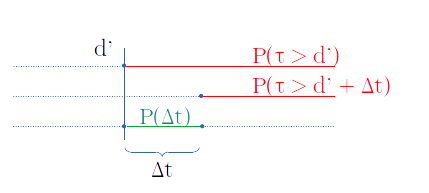
\includegraphics[width=0.75\linewidth]{timeline.png}
\end{center}

\section{Bonds}\label{bonds}

A bond is an instrument that represents a loan made by an investor to a
borrower (typically corporate or governmental). Bonds are used by
companies, municipalities, states, and sovereign governments to finance
projects and operations. Owners of bonds are debt-holders, or creditors,
of the issuer. Bond details include the end date when the principal of
the loan is due to be paid to the bond owner and usually includes the
terms for variable or fixed interest payments made by the borrower.

The coupon is the interest rate that the issuer pays to the holder.
This rate can be fixed throughout the life of the bond but it can also
vary with a money market index, such as LIBOR, or it can be even more
exotic.

\subsection{Pricing}\label{pricing}

The price of a bond can be computed as the present discounted value of
future cash flows generated by the bond itself.

For example consider a 3-years bond with a face value of 100 EUR
providing coupons at a 6\% rate annualy. Assume also that the interest
rates are 5.0\% 5.8\% 6.4\% and 6.8\% for 1, 2, 3, 4 year maturities. To
compute the present value of the first copuon we need to discount it at
5.0\% for 1 year, for the second the discount has to be at 5.8\% and so
on. The price will be then:

\[6e^{-0.05\times 1}+6e^{-0.058\times 2}+106e^{-0.064\times 3} = 98.53~\textrm{EUR}\]

    \begin{tcolorbox}[breakable, size=fbox, boxrule=1pt, pad at break*=1mm,colback=cellbackground, colframe=cellborder]
\prompt{In}{incolor}{6}{\boxspacing}
\begin{Verbatim}[commandchars=\\\{\}]
\PY{k+kn}{from} \PY{n+nn}{math} \PY{k}{import} \PY{n}{exp}
\PY{n}{rates} \PY{o}{=} \PY{p}{[}\PY{l+m+mf}{0.05}\PY{p}{,} \PY{l+m+mf}{0.058}\PY{p}{,} \PY{l+m+mf}{0.064}\PY{p}{,} \PY{l+m+mf}{0.068}\PY{p}{]}

\PY{n}{N} \PY{o}{=} \PY{l+m+mi}{100}
\PY{n}{maturity} \PY{o}{=} \PY{l+m+mi}{3}
\PY{n}{fixed\PYZus{}coupon} \PY{o}{=} \PY{l+m+mf}{0.06}
\PY{n}{price} \PY{o}{=} \PY{l+m+mi}{0}
\PY{k}{for} \PY{n}{tau} \PY{o+ow}{in} \PY{n+nb}{range}\PY{p}{(}\PY{l+m+mi}{1}\PY{p}{,} \PY{n}{maturity} \PY{o}{+} \PY{l+m+mi}{1}\PY{p}{)}\PY{p}{:}
    \PY{n}{price} \PY{o}{+}\PY{o}{=} \PY{n}{N} \PY{o}{*} \PY{n}{fixed\PYZus{}coupon} \PY{o}{*} \PY{n}{exp}\PY{p}{(}\PY{o}{\PYZhy{}}\PY{n}{rates}\PY{p}{[}\PY{n}{tau}\PY{o}{\PYZhy{}}\PY{l+m+mi}{1}\PY{p}{]} \PY{o}{*} \PY{n}{tau}\PY{p}{)}

\PY{n}{price} \PY{o}{+}\PY{o}{=} \PY{n}{N} \PY{o}{*} \PY{n}{exp}\PY{p}{(}\PY{o}{\PYZhy{}}\PY{n}{rates}\PY{p}{[}\PY{n}{maturity} \PY{o}{\PYZhy{}} \PY{l+m+mi}{1}\PY{p}{]} \PY{o}{*} \PY{n}{maturity}\PY{p}{)}
    
\PY{n+nb}{print} \PY{p}{(}\PY{l+s+s2}{\PYZdq{}}\PY{l+s+si}{\PYZob{}:.2f\PYZcb{}}\PY{l+s+s2}{ EUR}\PY{l+s+s2}{\PYZdq{}}\PY{o}{.}\PY{n}{format}\PY{p}{(}\PY{n}{price}\PY{p}{)}\PY{p}{)}
\end{Verbatim}
\end{tcolorbox}

    \begin{Verbatim}[commandchars=\\\{\}]
98.53 EUR
    \end{Verbatim}

 \subsection{Implied Probability of Default on Coupon Bonds}\label{default-probabilities-and-bond-prices}

The price of a bond issued by a party is directly linked to the credit
rating of that party, since there is always a default risk associated
with a bond, which means that the borrower might not be able to pay the
full or partial amount of the loan taken. So, bonds with low ratings,
called junk bonds, are sold at lower prices and those with higher
ratings, called investment-grade bonds, are sold at higher prices.

We can then estimate the probability of a company default directly from
the prices of the bonds issued by it. You can imagine that the spread
between a corporate bond over the risk-free rate should compensate for
the loss in case of default, so naively:

\[\lambda = \frac{s}{1-R}\]

In a more detailed way let $X$ represent the present value of a bond cash flow stream. When you
have a default probability then $X$ becomes a random variable with a range
of possible values. The way
to value the bond in this case is to take each possible value of $X$, multiply it
by its probability and sum the results. In other words the value of the bond
should equal the mathematical expectation of $X$.

To illustrate the idea, consider the case of a bond with 4 coupon payments
until maturity. Let $p$ be the probability that the bond survives from one
coupon payment to the next and let $X_i$ ($i$ = 0, 1, 2, 3, 4) be the value of
$X$ given that the bond defaults after making its $i$-th coupon payment. 
The expectation of $X$ can then be expressed as:

\begin{align*}
\mathbb{E}(X) &= X_0(1-p) + X_1 p(1-p) + X_2 p^2 (1-p) + X_3 p^3 (1-p) + X_4 p^4 \\
&= X_0 + (X_1 - X_0)p + (X_2 - X_1)p^2 + (X_3 - X_2)p^3 + (X_4 - X_3)p^4
\end{align*}

Assuming a constant recovery value $R$ the values $X_i$ are:

\begin{align*}
X_0 &= RN \\
X_1 &= (C + RN)/D \\
X_2 &= C/D + (C + RN)/D^2 \\
X_3 &= C/D + C/D^2 + (C + RN)/D^3 \\
X_4 &= C/D + C/D^2 + C/D^3 + (C + N)/D^4 \\
\end{align*}

Substituting into the expectation formula:

\begin{align*}
\mathbb{E}(X) &= C((p/D) + (p/D)^2 + (p/D)^3 + (p/D)^4) + \\
&RN(1-p)(1+(p/D)+(p/D)^2 + (p/D)^3) + \\
&N(p/d)^4 
\end{align*}

It is now easy to generalise to the case of $N$ coupons:

\[ \mathbb{E}(X) = C \sum_{k=1}^{N}{(p/D)^k} + RN(1-p)\sum_{k=1}^{N-1}{(p/D)^k} + N(p/D)^N \]

Each of the sums in this s formula is a geometric series that can be collapsed
into a single term. The formula for collapsing a general geometric series is 

\[ \sum_{k=0}^N a^k = 1 + a + a^2 + \ldots + a^N = \cfrac{1-a^{N+1}}{1-a} \]

Hence we get:

\begin{align*}
\mathbb{E}(X) &= C(p/D) \cfrac{1-(p/D)^N}{1-(p/D)}+RN(1-p)\cfrac{1-(p/D)^N}{1-(p/D)} + N(p/D)^N \\
&= \Big(C(p/D) + RN(1-p)\Big)\cfrac{1-(p/D)^N}{1-(p/D)} + N(p/D)^N 
\end{align*}

With $\mathbb{E}(X)$ equal to the price of the bond, this equation can be solved numerically for the 
survival probability $p$.

To get the default probability for the bond, simply subtract the survival
probability from 1, default probability =~$1 - p$. The cumulative default
probability, or the probability that the bond defaults anytime within the
next $n$ coupon periods is $(1 - p)^n$.

There are several ways to test the formula for logical consistency. First look
at the case where the survival probability is zero so that with $p = 0$ the
formula reduces to:

\[\mathbb{E}(X) = RN\]
this is logical since when default is immanent the price should just equal the
recovery amount.
In the case where survival is certain and the risk free rate is zero you have
$p = 1$ and $D=1$:

\[\mathbb{E}(X) = NC + F \]
The price here is equal to the total of the coupon payments plus the face
value, as you would expect.
